\documentclass{article}
\usepackage{amsmath}
\usepackage{amssymb}
\usepackage{amsfonts}
\usepackage{mathrsfs}
\usepackage{float}
\usepackage{fancyhdr} % For custom headers and footers
\usepackage{geometry} % For page layout
\geometry{a4paper, margin=1in}

\usepackage{tikz} % for game tree visualizations
\usetikzlibrary{trees, positioning, calc, fit}

\pagestyle{fancy} % Activate the fancyhdr package
\fancyhf{} % Clear all header and footer fields

\fancyhead[R]{\textbf{Saggese \thepage}} % Right-aligned text
\renewcommand{\headrulewidth}{0.4pt} % custom width of header line


\begin{document}

\begin{titlepage}
    \centering
    \vspace*{1in} 
    {\Large Problem Set 3} \\[1.5cm] % Subtitle


    {\Large \textbf{Allegra Saggese}} \\[0.5cm] % name
    {\large Microeconomics 204B} \\[1.5cm]

    {\large Friday, March 21 2025} \\ [.5cm] % Display today's date - tbd 
    {\small \textit{Please note ChatGPT was used to convert handwritten notes to LaTeX, or to summarize handwritten mathematical steps for ease of reading .}}
    \\[2cm] 

\end{titlepage}

\section{Problem 1}
\subsection*{(a)}

\begin{itemize}
    \item The best response function when $v \in (c+2t, c+3t)$ can be found by solving the FOCs of the KKT
    \item recall $M = v - (p_j + td)$
    \item Firm 1's demand function is $(p-c)q = M \hat{z}$, so $ \implies (p-c)q = v - (p_j + td)$
    \item $M \hat{z} = v - p_j + td$ for all $j = 1, 2$
    \item so we start by looking at the cost of buying, and solving for z: 
    \[
    p_1 + tz < p_2 + t(1-z) 
    \]
    \[
    tz < (p_2 + t - tz - p_1) / 2t
    \]
    \[
    2tz > (p_2 + 2 - p_1)
    \]
    \[
    z = (p_2 + t - p_1)/2t
    \]
    At $z$, the consumer is indifferent between which firm to buy from either firm because they're equal distance. Below we generalize from 1,2 to $i,j$:
\end{itemize}


\[
\max_{p_j} (p_j - c) \cdot (\overline{p}_{-j} +  p_j) \cdot (M/2t)
\]

taking the first order condition: 

\[
(t + p_{-j} + c - 2p)(M/2t)
\]

where, from the first order condition we get the following conditional equalities: 
\[
\left\{
  \begin{array}{ll}
    \leq 0 & \text{if } p_j = \overline{p}_{j} - t\\
    = 0 & \text{if } p_j \in [\overline{p}_{-j} - t, \overline{p}_{-j} +t]\\
    \geq 0 & \text{if } p_j = \overline{p}_{j} + t
    \end{array}
\right.
\]

\begin{itemize}
    \item given that $p_{-j} = c + 3t$, then $t + \overline{p}_{-j} + c - 2p_j \leq 0$
    \item when $\overline{p}_{-j} \in [c - t, c+3t]$ then $ t + \overline{p}_{-j} + c - 2p_j \geq 0$
\end{itemize}

Best response functions are the following:

\[
\left\{
  \begin{array}{ll}
    p_{-j} + t & \text{if } \overline{p}_{j} \leq c - t\\
    (1/2)(\overline{p}_j + c) & \text{if } p_j \in [c-t, c+3t]\\
    \overline{p}_j + t & \text{if } \overline{p}_j \geq c + 3t
    \end{array}
\right.
\]


\subsection*{(b)}
Now firms max profit, where $x$ is the inverse demand, such that: 
\[
\max_{p_i} (p_i - c) \cdot x_i(p_i, p_j^*) = (p_i - c) \cdot \frac{t + p_j^* - p_i}{2t} M
\]

and for $v \in (c + t, (3/2)t)$ then $ v > c + t + (1/2)t = v > c + (3/2)t$ so in equilibrium it holds. Here the unique nash equilibrium is $p_i = p_j = c + t $

\subsection*{(c)}
from above 
\[
v - p_i - t\, z_i = 0 \quad \Longrightarrow \quad z_i = \frac{v - p_1}{t}.
\]
If $0 \le z_1 \le 1$, then consumers on $[0, z_1]$ buy from firm 1. The same holds with symmetry for firm 2. Firms are competing for the middle of the market, often, and try to max their own profit. 
\\
If both firms $i, j$ chooses $p_i, p_j$ to maximize profits, then:
\[
\pi_i = (p_i - c)q = v - (p + tz_i) 
\]

so, rearranging gives us: $z_i = \tfrac{v - p_i}{t}$ (assuming $0 \le z_i \le 1$) and profits are equivalent to:
  \[
  \pi_i = (p_i - c)\,z_i = (p_i - c)\,\frac{v - p_i}{t}.
  \]

The same is true for firm 2 because of symmetry so I won't repeat the functions. Then, we rearrange and take the profit, and differentiate to get the FOC for the optimal price for the firm: 
\[
\pi_i = \frac{1}{t}\,\bigl[(p_i - c)(v - p_i)\bigr].
\]
\[
\frac{d\pi_i}{dp_i} = \frac{1}{t}\bigl[v - 2p_i + c\bigr] = 0
\quad\Longrightarrow\quad p_i^* = \frac{v + c}{2}.
\]


Where the same holds for the other firm, where $p_i^* = \frac{v + c}{2}$. So, in equilibrium:
\[
(\frac{v +c}{2}, \frac{v + c}{2}) = (p_i^*, p_j^*)
\]

With the initial constraint: $v < c + t \implies$ some consumers will not buy because there would be negative utility if they are too far from either firm, such that their value is less than their utility less their cost. 

\[
z_i = \frac{v - p_i^*}{t} = \frac{v - \frac{v + c}{2}}{t} = \frac{v - c}{2t}, 
\quad
z_j = 1 - \frac{v - p_j^*}{t} = 1 - \frac{v - \frac{v + c}{2}}{t} = 1 - \frac{v - c}{2t}.
\]
Since $v < c + t$, we have $v - c < t$, so
\[
\frac{v - c}{2t} < \frac{t}{2t} = \frac{1}{2},
\]

\[
z_1 < \frac{1}{2} < z_2.
\]

Only consumers that are in the distance of $[0, z_i]$ buy from firm 1 and similarly those who are on the interval $[z_j, 1]$ buy from firm 2 - there is an area of no market reach. 

\subsection*{(d)}

When $v \in (c + t, c + (3/2)t)$ there exists a unique equilibrium such that $p_1 = p_2 = v - t /2$ in equilibrium. This occurs when $ v > c + t$, which we will compare to the above case where $ v < c + t$. Recall that if $v$ is greater than cost and transportation, then consumers are willing to buy. If this holds for all consumers, then firms will set the distance equivalent to each other and share the profits. This is one potential way to play the game, and results in equilibrium output where $p_1^* = p_2^* = v - t /2$.
\\
We can show this by taking the FOC of the profit maximizing function, and rearranging for $v$:

\[
\frac{d(p_i - c)x_i(p_i, p_j)}{dp_i} = \frac{d(p_i - c)(v-p_i)\cdot(M/t)}{dp_i} = (t + p_j + c)(M/2t) \geq 0
\]

If you rearrange, and plug back in for $v$ we get: $p_i&* = v - t /2 $. In addition to this equilibrium, which is symmetric for both $i,j$, there is an asymmetric equilibrium in this case, because firms can deviate by a small amount, $\epsilon$ in order to capture customers from the other firm. This is because there are multiple equilibria possible in this Bertrand price competition, and its also why firms can only \textit{lower} prices and cannot raise them, or they risk losing customers all together where costs exceed the value from the product. 


\subsection*{(d)}

As travel costs decrease, more consumers will enter the market, or may change where they buy something (i.e. which firm they buy from). Therefore, firms can increase price (cost for consumers) and raise prices slightly. Overall, profits should stay above competitive prices for each firm. 

\section{Problem 2}
\subsection*{(a)}
For a change of cost in production, we see that $\delta \geq 1/2 \implies p \in [c, p^m]$ is a subgame perfect nash equilibrium. If costs change, $p \in [c, p^m] \rightarrow p \in [c', p^m]$. 

\begin{itemize}
    \item Where $c' > c$ the profitable strategies decrease in numbers (quantity)
    \item $c' < c$ the number of profitable strategies rise
\end{itemize}
\\
The lowest price possible to ensure that profits remain positive will change and the monopoly's price, $p^m$ will increase. But, the most profitable price (cost) is the upper bound, so it does change where $\delta \geq 1/2$, so $p^m$ shifts up by the change in cost. Overall profits will decrease if firms are not already selling at $c$. 

\subsection*{(b)}
If there is a permanent change in period 2, we need to look at the profits, assuming there are two firms. If profits of firm 1 are greater than 1/2 of the profits of firm 2 ($\pi_1 > \pi_2/2$), then firm 1 could deviate in $t=1$ to take all the profits, then take in zero profits for the future periods. This is profitable where the deviation is greater than the summation of NPV payoffs in the future. 
\\
\\
If $\pi_1 \approx \pi_2/2$ the change in cost will only lead them to cooperate. 

\section{Problem 3}

\subsection*{(a)}

$\lambda \in (0,1)$ \\
$\lambda \rightarrow x(p) \rightarrow p_h$ \\
$(1-\lambda) \rightarrow \alpha x(p) \rightarrow p_l$ \\
\\
When $\delta$ is sufficiently high, then $p_h = p_l = p^m$ \\
The monopoly price is sustained \textit{if and only if} the present value of future losses is large enough, relative to the possible current gain from deviation. The losses would be foregone earnings achieved by undercutting the rival firms. \\
\\
Firms collect $1/2 \cdot \pi_i$ if $p_h = p_l = p^m$ in equilibrium, so:
\[
\text{Expected value }= \beta[(1-\lambda)\pi_l + \lambda \pi_h] \div 2
\]
\[
\text{where } \beta = \frac{\delta}{1-\delta} \text{ because } \delta^i = \delta^1 + \delta^2 + \delta^3...
\]
So in the high cost (and also low-cost scenario), firms deviate, where: 
\[
\pi_h/2 = \beta[(1-\lambda)\pi_l + \lambda \pi_h]/2
\]
\\
In equilibrium, we can take the firm's profit maximization, and plug in the the profit margin, where $p^m - c$ is equal to the price. We look first at solving for the demand for high demand firms.
\[
[p_l\cdot \alpha x(p_l) - \lambda(p_l\cdot \alpha x(p_l)] = \pi_l \implies (p^m - c)\alpha x(p_l) - \lambda(p^m -c)\alpha x(p_l) = \pi_l
\]
\[
(p^m -c)\alpha x(p^m) = \alpha \pi_l
\]
so expected value is: 
\[
\beta[(1-\lambda)\alpha - \lambda] = \pi = (1-\delta)
\]
\[
\pi/\pi = (\delta/(1-\delta))(\lambda + (1-\lambda)\alpha) = 1
\]
Now, for low demand firms, we get a similar result:
\[
\alpha = (\delta/(1-\delta))(\lambda + (1-\lambda)\alpha)
\]
Which keeps firms from cooperating. If we want to find the correct value of $\delta$, then we need to solve for delta from these equations: 
\[
(1-\delta) = \delta\lambda + (1-\lambda)\alpha\delta
\]
\[
-\delta = \delta\lambda +\alpha\delta - \lambda\alpha\delta - 1
\]
\[
\delta \geq 1/(1 + \lambda + (1-\lambda)\alpha)
\]
So when $\delta \geq 1/(1 + \lambda + (1-\lambda)\alpha)$, where $\alpha \in [0,1]$ then $p_l = p_h = p^m$. We need $\delta \geq (1/2)$ for this to hold. 

\subsection*{(b)}

For sustainable prices in both periods, we solve out for the value of delta, such that it is $\delta = 1/(1 + \lambda + (1-\lambda)\alpha)$. But, if $\pi_{h,t-1} > [\delta/(1-\delta)][\pi_{h,t}/2]$ then a firm will deviate. When $\delta < \underline{\delta}$, where $\underline{\delta}$ is the minimum value of the discount rate needed to sustain monopoly pricing, we will calculate the profits: 
\[
\pi_h = \beta[px(p)-c]
\]
\[
(\pi_h - \delta\pi_h) = \delta(px(p)-c) \implies \pi_h = \delta[(p\cdot x(p) - c + \pi)]
\]
\[
\pi_h \geq \frac{(1-\lambda\cdot\pi_l)}{(1-\delta)} \implies \delta \leq \frac{(1-\lambda)\pi_l - \pi_h}{(1-\lambda)\pi_l}
\]
So if it is more profitable to deviate in the high demand state, then price in low demand stays at monopoly pricing, while the price in a high demand state will drop. 

\subsection*{(c)}
When $\delta < 1/2 \implies p_l = p_h = c$. This is because, any SPNE outcome path when $\delta < 1/2$ muat have all sales occurring at cost, c. Let's look at the value function, such that: 
\[
V_{jt} = \sum_{\tau \geq t}\delta^{\tau-1}\pi_{jt} \text{ , with definition: } \pi_t = \pi_{1t} + \pi_{2t}
\]
\[\pi_t \leq V_{jt} \text{ for } j = 1,2 \text{ and every }t 
\]
From this, we can see that each firm can get a profit very close to $\pi_t$ when they undercut their rivals by just a tiny amount, $\epsilon$. \\
\\
Now we consider (1) when $\pi_t > 0$. There is also another period, $\tau$ such that $\pi_{\tau} > 0$, and  $\pi_{\tau} > \pi_{t}$ for all $t$. When $t = \tau$, then we have $2\pi_{\tau} \leq (V_{1\tau} + V_{2\tau}) \rightarrow V_{1\tau} + V_{2\tau} \leq \frac{1}{1-\delta}\pi_{\tau}$. But we know that, given the value of $\delta$ that $\frac{1}{1-\delta}\pi_{\tau} < \pi_{\tau}$.  \\ 
\\
By contradiction, this cannot hold when $\delta < 1\2$. Therefore, the requirements for a repeated choice game with an SPNE cannot hold for the monopoly price, and therefore prices must be equal to costs, or else the inequalities between profit and discounted value are contradicted. \\
\\
If we also consider (2) the case where for any period, $t$, there is some period, $\tau > t$ such that $\pi_{\tau} > \pi_t$, then we can define $\tau(t)$ for $t \geq 1$ such that $\tau(1) = 1$ and for $t \geq 2$, then 
\[
\tau(t) = Min\{ \tau > \tau(t-1): \pi_tau > \pi_{\tau(t-1)} \} \quad \text{ where } \pi^m = (p^m - c)x(p^m)
\]
With the monopoly profit level, we know that the profit function is increasing in time, and therefore must converge to its limit, $\overline{\pi} \in [0, \pi^m]$, the monopoly price. But, notice that all the other profits, as a function of $\tau(t)$ must still respect the inequality $2\pi_{\tau(t)} \leq V_{1,\tau(t)} + V_{2,\tau(t)}$ for all $t$ So, at the monopoly price we have:
\[
V_{1,\tau(t)} + V_{2,\tau(t)} \leq \frac{1}{1-\delta}\overline{\pi} \implies 2\pi_{\tau(t)} \leq \frac{1}{1-\delta}\overline{\pi}
\]
Ad therefore, when $\delta < 1/2$ this condition is clearly violated as $t \rightarrow \infty$ (or gets sufficiently large and therefore close to the monopoly profits). 

\section{Problem 4}
\subsection*{(a)}

To find the pooling equilibrium, where \textit{I} bids and \textit{U} responds, we need to find the PBE where $x_a = x_b$. Where the payoffs are:
\[ 
U = x_a, x_b \qquad I= 10, 110 \]

Look first at good a, where if type a:
\[
\left\{
  \begin{array}{ll}
    x_a - 120 = & 100 - x_a\\
    2x_a = & 220 \\
    x_a = & 100
    \end{array}
\right.
\]
Given this we see $x_a$ has a max value. Let's keep going. 
\[
120\mu + (1-\mu)60 = \mathbb{E}[value]
\]
\[
1/2*120 + 1/2*60 = 90 = \mathbb{E}[\theta]
\]
So, \textit{U} has an expected value of $\theta$ of 90. \textit{I} is willing to bid up to 100 to get $a$, so the value of $x$ is: $90 \leq x \leq 100$. This is the \textbf{pooling equilibrium} $U$ will accept the bid. When $\mu < 1/2$, and $x < 90$, then \textit{U} will reject. 


\begin{center}
    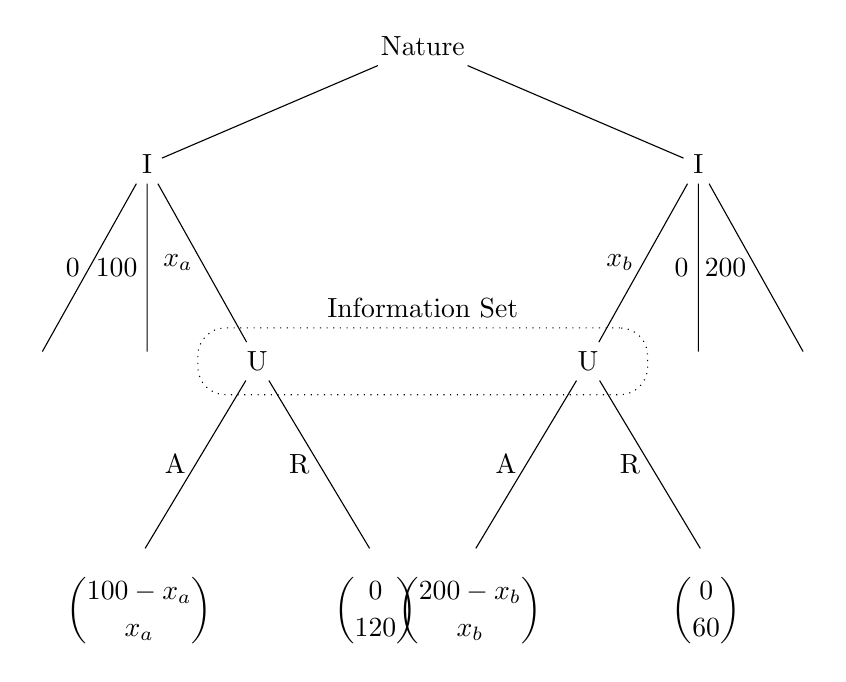
\begin{tikzpicture}[
    level 1/.style={sibling distance=70mm},
    level 2/.style={sibling distance=14mm, level distance = 25mm},
    level 3/.style={sibling distance=30mm, level distance = 25mm},
    grow=down]
    % Root node
    \node {Nature}
        child { node {I} 
            child { node {} edge from parent node[left]{$0$} }
            child { node {} edge from parent node[left]{$100$} } 
            child { node(a3) {U}
                child {node [label=below:{$\displaystyle\binom{100-x_a}{x_a}$}] {}edge from parent node[left]{A}}
                child {node [label=below:{$\displaystyle\binom{0}{120}$}] {}edge from parent node[left]{R}}
                edge from parent node[left]{$x_a$}
                }
            }
        child { node {I} 
            child { node(b3) {U} 
                child {node [label=below:{$\displaystyle\binom{200-x_b}{x_b}$}] {}edge from parent node[left]{A}}
                child {node [label=below:{$\displaystyle\binom{0}{60}$}] {}edge from parent node[left]{R}}
                edge from parent node[left]{$x_b$}
                }
            child { node {}edge from parent node[left]{$0$} }
            child { node [] {}edge from parent node[left]{$200$} } 
            };
    % Draw a dotted rectangle around nodes a3 and b3
    \node[draw, dotted, fit = (a3) (b3), inner sep=5mm, inner ysep=1.8mm, label={Information Set}, rounded corners =10] {};

\end{tikzpicture}
\end{center}

\subsection*{(b)} 

Where $x_a \neq x_b \implies x_a $ rejects and $x_b$ accepts. Starting with a:
\[
x_a \geq 120 \text{ to accept } U \qquad x_a \leq 100  \text{ to bid } I
\]
Now b:
\[
x_b \geq 60 \text{ to accept } U \qquad x_b \leq 200  \text{ to bid } I
\]
So the seperating equilibrium is:
\[
0 \leq x_a \leq 100 \leq x_b \leq 200 
\]
Here, if $x \in [100,200] $ type b will accept. Given that there is signalling, no outcomes where $x_a$ are accepted and $x_b$ are rejected exist. So our final outcomes are: 
\[
x_a \rightarrow (x_a \leq 100, \text{ reject }, \mu_u(a|x_a)=1)
\]
\[
x_b \rightarrow (100 \leq x_b \leq 200, \text{ accept }, \mu_u(b|x_b)=1)
\]

\subsection*{(c)}

When \textit{I} plays $x_b \in [101,200]$, it is obvious that for type b this is still within range, but it is weakly dominated because with $x_b = 100$, player \textit{U} accepts the bid. In a refined PBE, we have $\{x_a \leq 100, x_b \leq 101, reject, \mu_u(a|x \leq 100) = 1\}$

\section{Problem 5}

\subsection*{(a)}
We are looking at positive selection where $r(\theta) \geq \theta$ for all $\theta \in [\underline{\theta}, \overline{\theta}]$ because $r(\cdot)$ is strictly decreasing. So we have the following: 
\begin{itemize}
    \item wage offer = $w$, and we have $w$ such taht $r(\theta) \leq w$ where the wage is accepted
    \item if $\theta' > \theta$ then $r(\theta') \leq w$ by definition, as the function of $r$ is decreasing
    \item so, all workers $\theta, \theta'$ will work at $w$
    \item thus if $\theta'$ is the ability, and it is greather than $\theta$ wage is set as $r(\cdot)$ is decreasing. 
\end{itemize}

\subsection*{(b)}

Because $r(\theta) > \theta$ for all $\theta$, we know that at $r(\overline\theta) > \overline\theta$ that no one will work because residual wages remain greater than $\overline{\theta}$ such that $\overline{\theta} = w$. If $\overline{\theta} = w$ then $w < r(\theta)$. This is also still pareto efficient, as all workers are receiving their maximum utility, which is the highest $\overline{\theta}$.

\subsection*{(c)}

\begin{center}
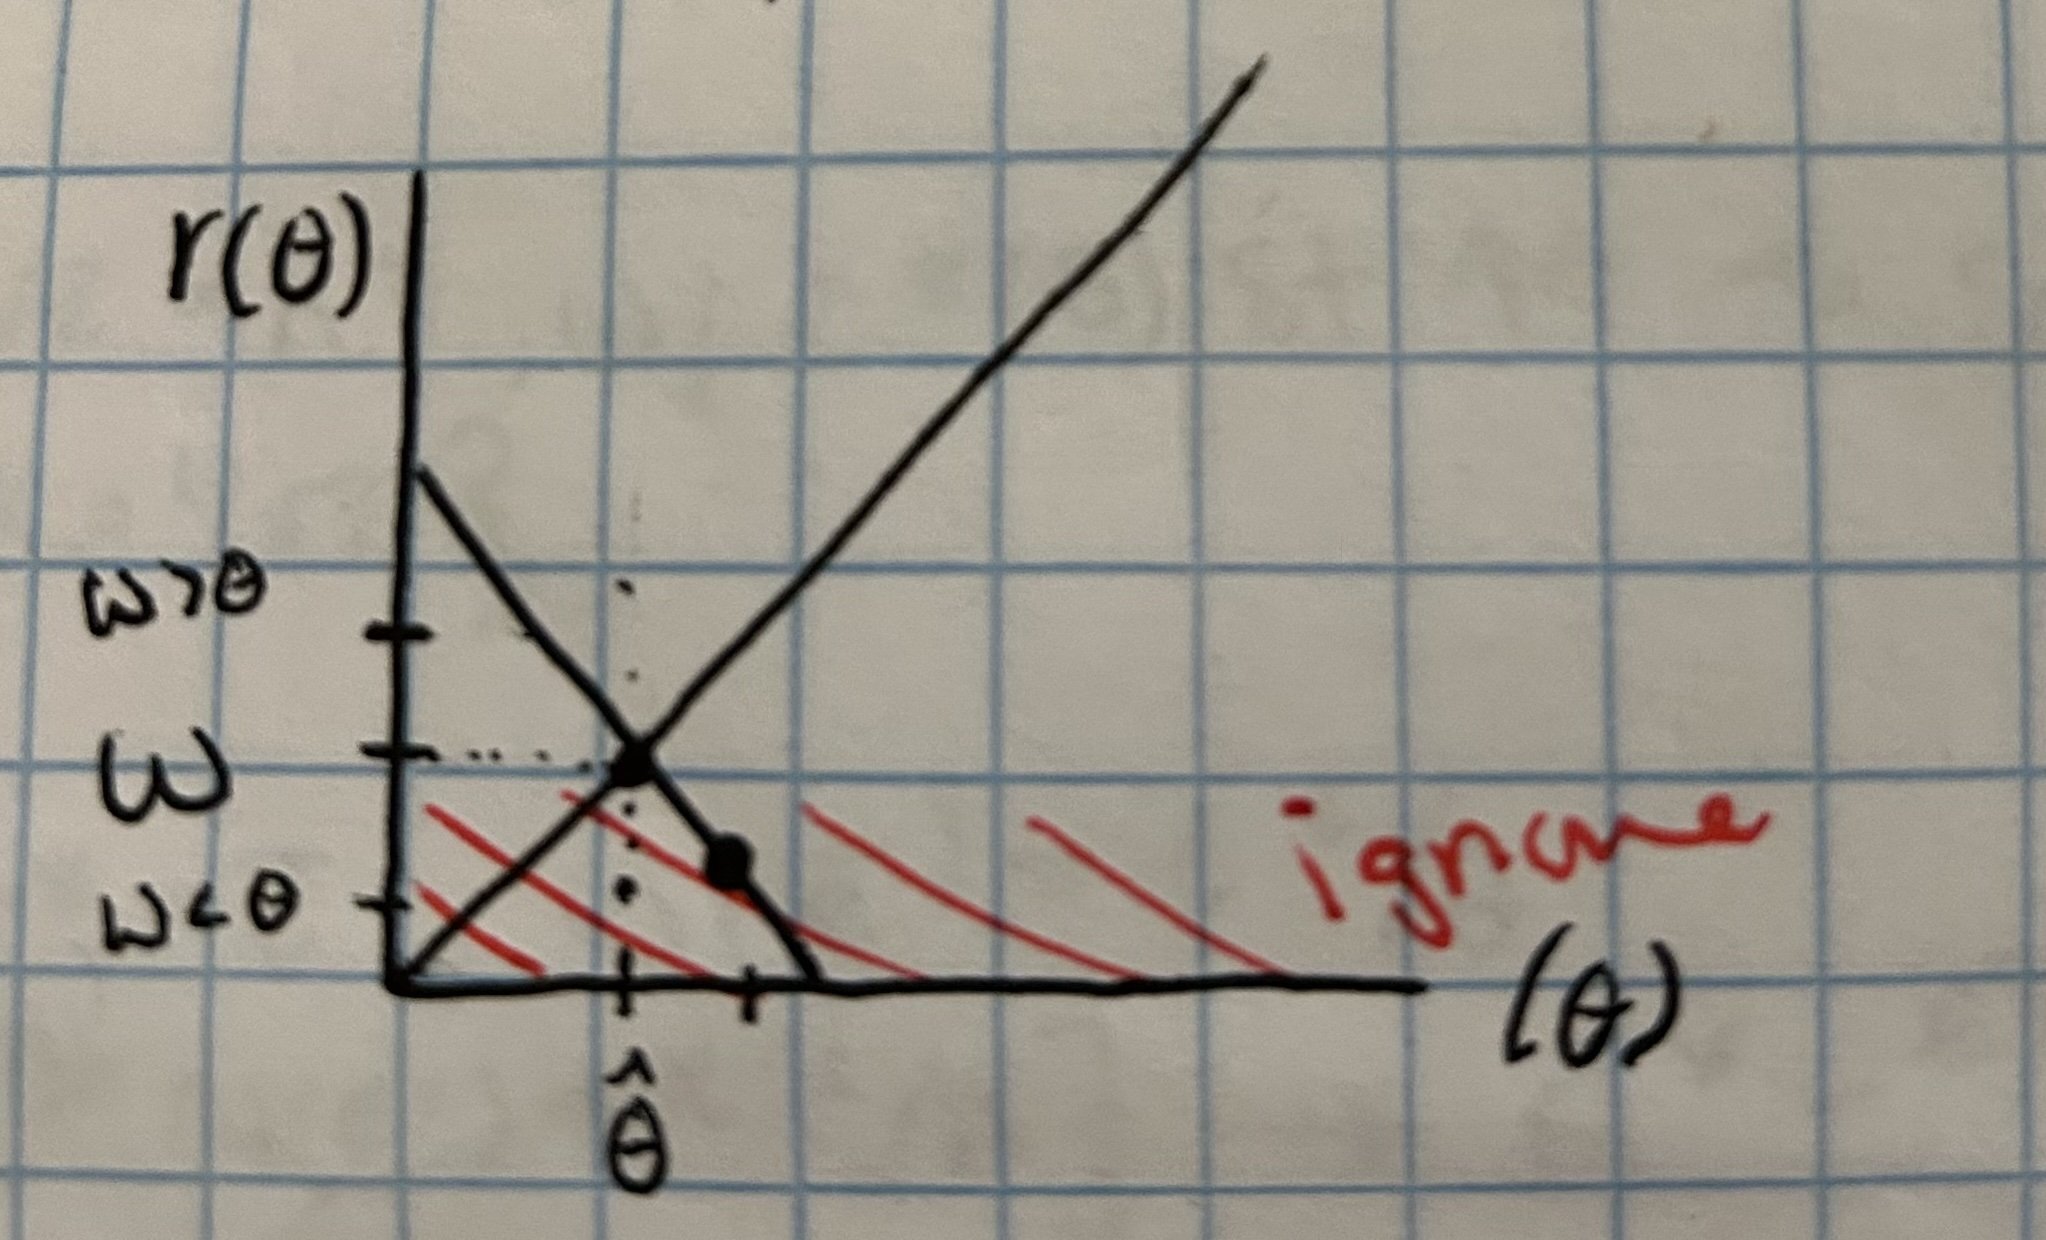
\includegraphics[width=.5\linewidth]{images/IMG_1835.jpg}    
\end{center}


We have $\theta$ s.t. $r(\theta) < \theta $ for $\theta > \overline{\theta}$ and $r(\theta) > \theta$ for all $\theta < \overline{\theta}$. We have the following results: 
\begin{itemize}
    \item if $w = \hat{\theta}$ only $\theta \geq \hat{\theta}$ work.
    \item if $w < \hat{\theta}$ only $\theta \geq \theta_w$ work, but in this case $\mathbb{E[\theta | \theta \geq \theta_w]} = w$ does not hold. 
    \item When $w > \hat{\theta}$ there will be some $\theta < \hat{\theta}$ that accept, and its not efficient.
\end{itemize}

Here we do not have a Pareto optimal outcome. 

\section{Problem 6}

\subsection*{(a)}

A Separating PBE is a monotonic function, with incentives for competition and consistency. We look at the separating PBE, where $[\underline{\theta}, \overline{\theta]}$, and:
\[
f(\theta) = +, \quad  c(e, \theta) = e^*(\theta)
\]
\[
w^*(e^*(\theta_H)) = \theta_H
\]
So for any $\theta' \implies w^*(e^*(\theta')) = \theta'$. So with workers, $\theta, \theta'$ and $\theta > \theta'$ then:
\[
\theta - \frac{e(\theta)^2}{\theta} \geq \frac{e(\theta')^2}{\theta'}
\]
This is incentive compatible. \\
\\
Now recall that $e^*(\theta) = k\theta$ if $k > 0$ and $\theta = w(e)$ such that $\frac{de}{\theta} = w'(e) = \frac{de}{w(e)} \implies 2e = w'(e)w(e)$. So we can now look at the workers’ utility maximization problem is the following.
\[
\max_e \ w(e) - c(e, \theta) = w(e) - \frac{e^2}{\theta}
\]
\[
FOC: \quad w'(e) - \frac{2e}{\theta} = 0
\]

Firms are competitive, such that: $w(e^*) = \theta$ in equilibrium. Therefore, $w'(e) = \frac{2e}{w(e)}$. It holds as such that $w(e) = \sqrt{2}e$. Additionally, with our value of $k = \frac{\theta}{2k\theta} = 1/2k = k$ we have that $k^2 = 1/2 \implies \frac{1}{\sqrt{2}} = k^*, e'^*(\theta) =  \frac{1}{\sqrt{2}}$. So the  separating PBE is $(e = \theta / \sqrt{2}, \ w(e) = \sqrt{2}e)$. The belief here is $\mu(\theta = \sqrt{2}e \mid e) = 1$.


\subsection*{(b)}
For the set of pooling equilibrium, we have two workers, $e^* = \overline{e}$ such that $w(\overline{e}) = \frac{\overline{e}^2}{\theta}$. We know: 
\[
\frac{\overline{e}^2}{\theta} > max[w(e') - \frac{\overline{e}^2}{\theta}] \rightarrow \overline{\theta}^* - \frac{\overline{e}^2}{\theta} \geq \theta - \frac{\overline{e}'^2}{\theta}
\]. So the pooling equilibrium is: 
\[
\{ e^* = \overline{e} | \overline{e} \leq \sqrt{\overline{\theta}^*(\theta - \overline{\theta})^*} \}
\]

\subsection*{(c)}

Assume $[\underline{\theta}, \overline{\theta}] = [1,2]$ and $f(\theta) = 1$
\begin{center}
    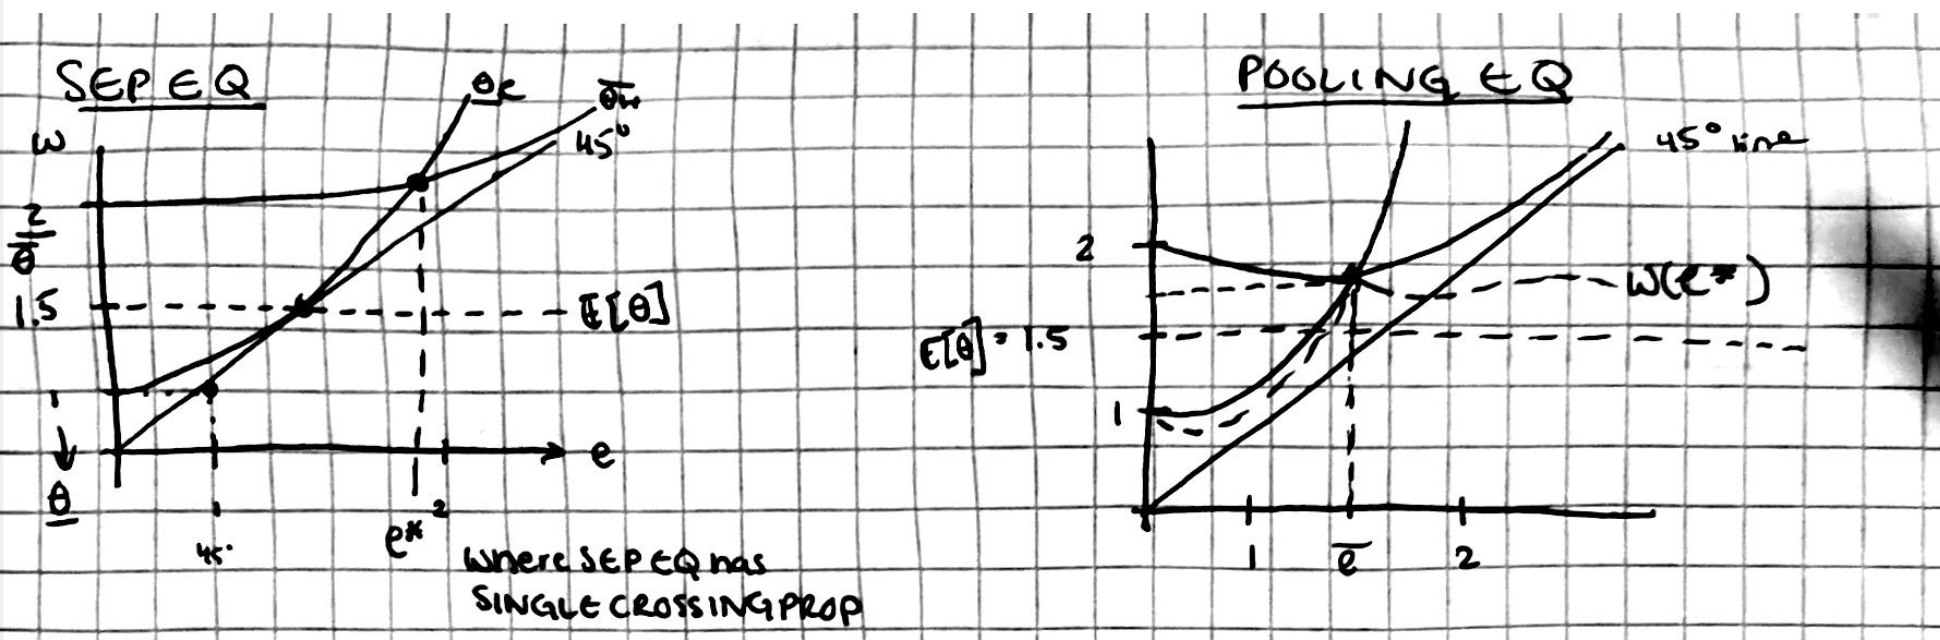
\includegraphics[width = .85\linewidth]{images/Screenshot 2025-03-22 at 20.52.48.png}
\end{center}

Intuitively in the separating equilibrium, we have that the value of $e^*$ is greater than the expected value of $\theta$, and as such there are two equilibrium for the high and low cost types. Here you can see its high types would accept $e^*$. While in the pooling equilibrium, all wages are set at $\overline{e}$ which is actually above the expected wage given $\theta$. These two diagrams are different in the sense that the actual wages vs. equilibrium points are different. In pooling equilibrium, you can aso see a hypothetical movement of the wage function, dependent on effort, $e$. 

\section{7}
\subsection*{(a)}

Effort is not observed here, so $e_2$ is not implementable. Start with the value function: 
\[
v(w) = \{ \sqrt{w} - g(E) | E=e_1 \} = \sqrt{w} - 4/3
\]

So $e_2$ should be preferable over the other levels of efforts, such that: 
\[
\begin{aligned}
&\textbf{(IC-1)}\quad
&&\frac{1}{2}v_{h} \;+\;\frac{1}{2}v_{\ell} \;-\;g(e_{2})
&&\;\;\ge\;\;\frac{2}{3}v_{h} + \frac{1}{3}v_{\ell} - g(e_{1}),
\\
&\textbf{(IC-2)}\quad
&&\frac{1}{2}v_{h} \;+\;\frac{1}{2}v_{\ell} \;-\;g(e_{2})
&&\;\;\ge\;\;\frac{1}{3}v_{h} + \frac{2}{3}v_{\ell} - g(e_{3}),
\\
&\textbf{(PC)}\quad
&&\frac{1}{2}v_{h} \;+\;\frac{1}{2}v_{\ell} \;-\;g(e_{2})
&&\;\;\ge\;\;0.
\end{aligned}
\]

From \(\textbf{(IC1)}: \quad\dfrac12v_{h} + \dfrac12v_{\ell} - 1.6 \;\;\ge\;\;\dfrac23v_{h} + \dfrac13v_{\ell} - \frac{5}{3}.\)

\[
3v_{h}+3v_{\ell} - 9.6
\;\;\ge\;\;
4v_{h}+2v_{\ell} - 10
\;\;\Longrightarrow\;\;
-v_{h} + v_{\ell} + {(10 - 9.6)}{\,0.4\,=\,2/5}
\;\;\ge\;\;0
\;\;\Longrightarrow\;\;
v{\ell}\;\ge\;v_{h}-\frac{2}{5}.
\]


From \(\textbf{(IC2)}: \quad\dfrac12v_{h} + \dfrac12v_{\ell} - 1.6 \;\;\ge\;\;\dfrac13v_{h} + \dfrac23v_{\ell} - \frac{4}{3}.\)
3v_{h}+3v_{\ell} - 9.6
\;\;\ge\;\;
2v_{h}+4v_{\ell} - 8
\;\;\Longrightarrow\;\;
v_{h} - v_{\ell} + \bigl(8 - 9.6\bigr)
\;\;\ge\;\;0
\;\;\Longrightarrow\;\;
v_{h} - v_{\ell} \;\ge\;1.6
\;\;\Longrightarrow\;\;
v_{h} \;\ge\;v_{\ell}+1.6.
v_{\ell}\;\;\ge\;v_{h}-\frac{2}{5}
\quad\text{and}\quad
v_{\ell}\;\;\le\;v_{h}-1.6.
\text{ But } \;(v_{h}-1.6)\; <\; (v_{h}-0.4)\. 

For all $v_{h}$, these constraints are contradictory.  No $(v_{h},v_{\ell})$ can satisfy them both.  

In order for $e_2$ to be implementable, then we need to solve for: 
\[
1/2v_h + 1/2v_l - g(e_2) \geq 2/3v_h + 1/3v_l - 5/3
\]

so solving down we get: 
\[
\frac{1}{6}v_h - g(e_2) \geq \frac{-1}{6}v_l - \frac{5}{3} + g(e_2) - 6 \implies v_h \leq v_l + 10 +6g(e_2)
\]
\[
v_h \leq v_l +10 +6(g(e_2)) \qquad v_h \geq v_l -8  +6(g(e_2))
\]

This results in:
\[
g(e_2) \leq \frac{3}{2}

\]

Only then does it get implemented. 

\subsection*{(b)}

Since \( e_{2} \) is not implementable at cost \( \frac{8}{5}\), implementation only occurs when: 
\begin{itemize}
    \item \( e_{1} \): Probability of high profit = \( \frac{2}{3} \), cost of effort = \( \frac{5}{3} \).
    \item \( e_{3} \): Probability of high profit = \( \frac{1}{3} \), cost of effort = \( \frac{4}{3}  \).
\end{itemize}

We are looking for where we can maximize expected profit against expected wage. We start with the wage $16/9$ and calculate the expected profits: 
\[
\pi(e_3) = 1/3*10 + 2/3*0 - 16/19 = 14/19
\]
Now for $e_3$ we can find the wages at both values (high and low) such that they satisfy both rationality and incentives, where we use: 
\[
\mathbb{E}[e_1 \text{ payoff }] = \mathbb{E}[e_3 \text{ payoff }]
\]

Solving it out we get $(w_h, w_l) = (4,1)$. 
\[
\pi(e_1) = 2/3*10 - 1/3*0 - 2/3*4 - 1/3*1 = 11/3
\]

Since $e_{2}$ is not implementable and $e_{3}$ yields much lower payoff, the optimal contract (from the principal’s standpoint) is to implement $e_{1}$. The value is set at $w_{h}=4, w_{\ell}=1$, where there is no incentive to deviate. 

\subsection*{(c)}

\begin{enumerate}
    \item If \( z > 1.5 \), then \( e_{2} \) is not implementable (same contradiction as above). Choice of either \( e_{1} \) or \( e_{3} \), but from above we know $e_1$ is preferred. So for all \( z > 1.5 \), the equilibrium effort is \( e_{1} \).

    \item If \( z \le 1.5 \), then \( e_{2} \) can be implemented (the constraints stop being contradictory). We can compare when the employer forces \( e_{1} \) versus the net payoff from forcing \( e_{2} \).

\begin{itemize}
    \item We know for \( z > 1.5 \), \( e_{2} \) is impossible, so \( e_{1} \) is used.
    
    \item Even for some \( z \le 1.5 \), we compare implement \( e_{1} \) and implement \( e_{2} \). Looking for a threshold: 
    \begin{itemize}
        \item If \( z > \bar{z} \), then \( e_{1} \) pays employees more.
        \item If \( z < \bar{z} \), then the employer prefers \( e_{2} \).
    \end{itemize}
\end{itemize}

So for values of z where $e_1$ is implementable we see: 
\begin{enumerate}
    \item If \( z > 1.5 \), cannot implement \( e_{2} \), $\implies$ \( e_{1} \).
    \item If \( z \le 1.5 \), choice of \( e_{1} \) or \( e_{2} \) depends on which yields higher net \( \Pi \), so we plug in $z$ for the expected payoffs and compare such that: 
\[
[z*10 - (1-z)*0] - w(z) = 0
\
\end{enumerate}


\section{Problem 8}

\subsection*{(a)}
See the drawing on the right for the proper spacing of the indifference curves and the value of $\hat{p}$
\begin{center}
    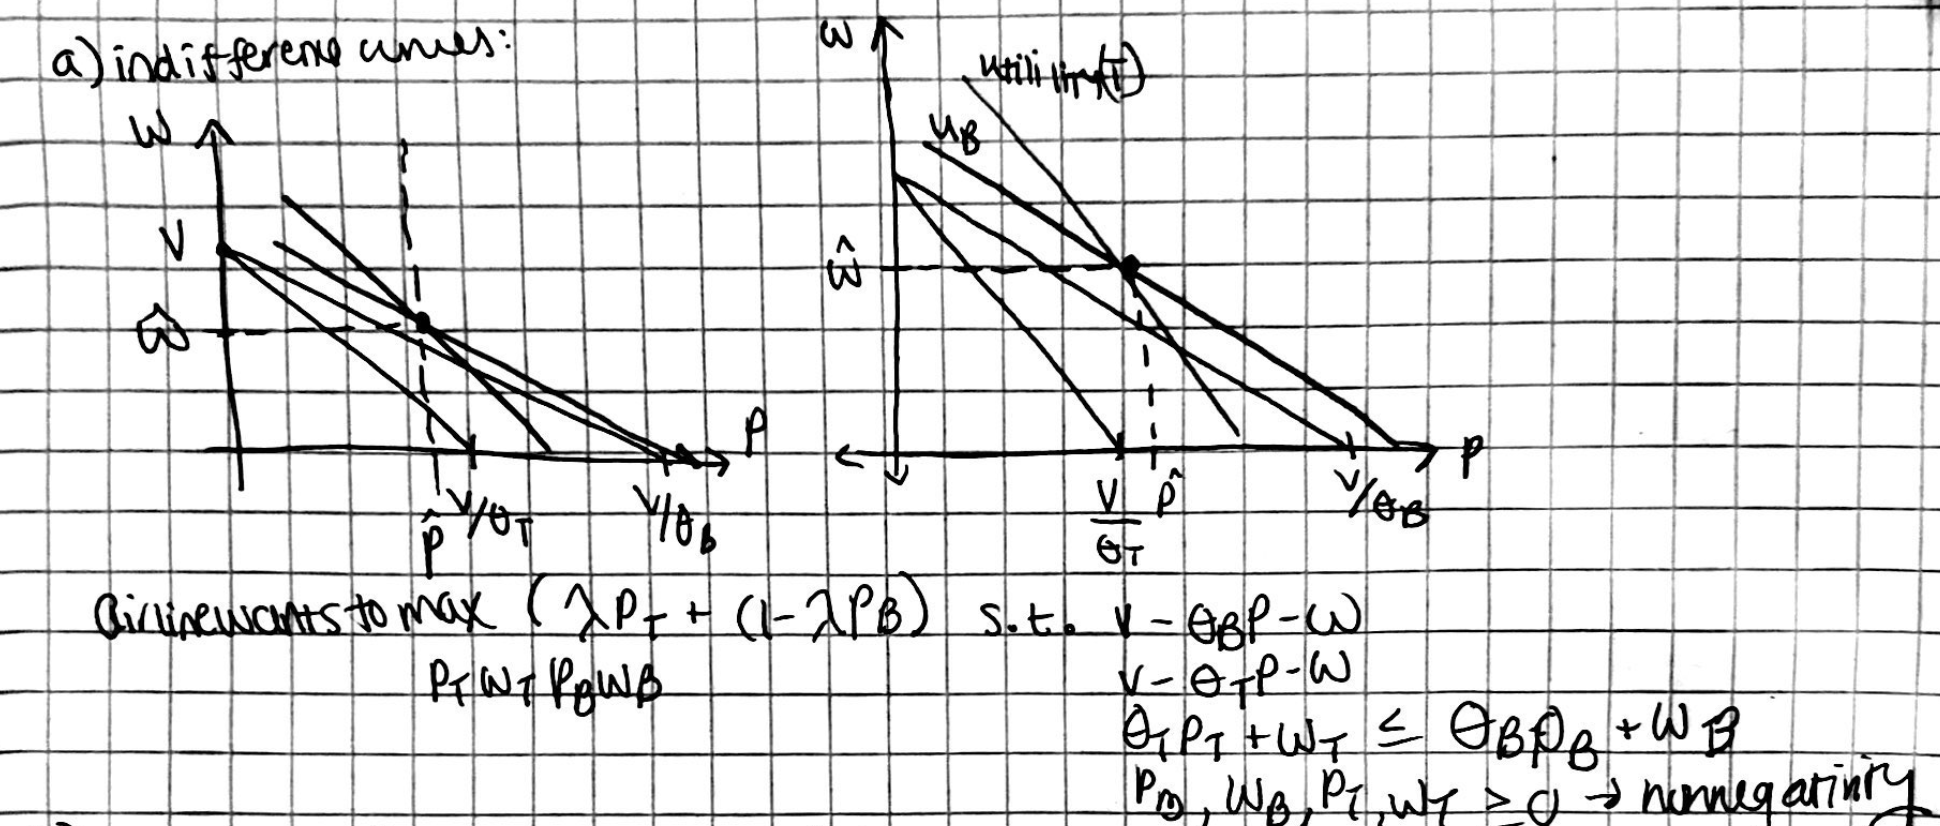
\includegraphics[width = .75\linewidth]{images/Screenshot 2025-03-22 at 20.53.04.png}
\end{center}

\subsection*{(b)}
From the constraints, we know that some tourists will be indifferent between buying and not buying a ticket, because some tickets to business travellers will possibly be equal to zero, given the final constraint of the problem on the graph. If that is possible, and the tourists have a type that indicates WTP for a ticket is always lower, than we can assume at some point, the willingness to pay for a ticket is zero by tourists. Therefore, there are some cases - possibly - in which a tourist is indifferent between buying and not buying a ticket. 

\end{document}